\section{Introduction}
Positioning devices are becoming increasingly popular in nowadays. For instances, telemetry chips on animals record animal herding histories; GPS equipment on cars records the vehicle movements; Mobile phones and wearable devices carried by people record pedestrians activities; Location-based web services (e.g., Foursquare, Facebook etc.) record user locations. These position data are often time-stamped and can be viewed as trajectories. Data analysis on trajectory data benefits a range of application area and services, including traffic planning, animal analysis, and social recommendations just to name a few. 

An important data analysis on trajectories is to discover co-moving objects. A \emph{co-movement} pattern~\cite{li2013managing} can be viewed as a set of objects that travel together for some duration. In practice, we can descritize the temporal domain of trajectories into snapshots, where each snapshot contains the geographical information of all objects. Formally, given a member size constraint $n$, a temporal constraint $k$, a \emph{co-movement} pattern is found when there exists a cluster with at least $n$ objects which appears for at least $k$ snapshots. Recent works have studied various co-movement patterns with different level of temporal constraints. Jeung et al. proposed \emph{convoy} pattern, which require the snapshots to be consecutive; Li et al. proposed \emph{swarm} pattern which relax the consecutiveness of snapshots and Li et al. proposed \emph{platoon} pattern which imposed a \emph{minimum local length} on the snapshots. We first provide a synthetic example to better illustrate these patterns in Figure~\ref{fig:related_work}, and the formal definitions are described in Section~\ref{sec:definition}.
\begin{figure} [h]
\center
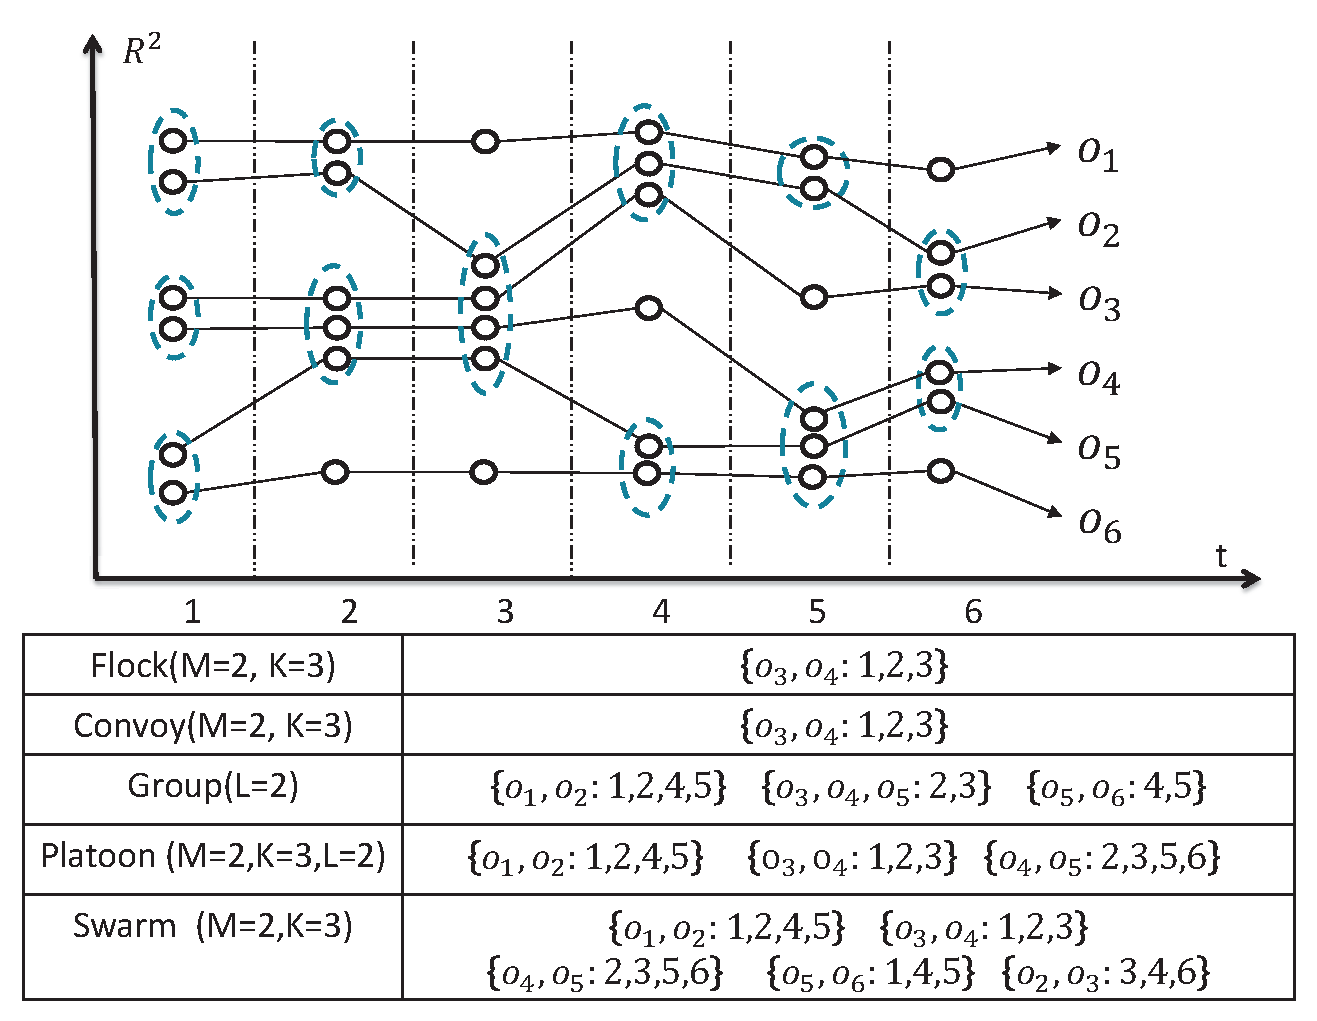
\includegraphics[width=0.5\textwidth]{related_work.eps}
\caption{Co-moving patterns in related works}
\label{fig:related_work}
\end{figure}

\begin{example}
Figure~\ref{fig:related_work} presents a hypothetical set of trajectories involving seven objects. Temporal domain is sliced into 5 snapshots. At each snapshot, objects belonging to the same clusters are marked in the same shape and color. Different patterns discovered are highlighted in the table. In particular:\\
\emph{Convoy} pattern requires the duration of a pattern to be \emph{consecutive}. In Figure~\ref{fig:related_work} only one convoy pattern is found, which is $\{o_3,o_4\}\{t_1,t_2,t_3\}$\\
\emph{Swarm} pattern relaxes the consecutiveness of duration, thus there are three patterns discovered.\\
\emph{Platoon} pattern requires that each local consecutive duration needs to have at least certain length, which is identified by the additional parameter $l$. When $l$ equals 2, there are two patterns discovered. Note that $\{o_6,o_7\}\{t_1,t_4,t_5\}$ is not included in the platoon pattern since $t_1$ is the local consecutive snapshot with duration 1, which is less than $l$.
\end{example}

We notice that, \emph{platoon} pattern is more general than \emph{convoy} and \emph{swarm}. This is because by setting appropriate $l$, \emph{platoon} can be reduced to \emph{convoy} and \emph{swarm} respectively~\cite{li2015platoon}. However, we observe that \emph{platoon} pattern is to loose on the temporal domain thus may result in less significant patterns. For example in Figure~\ref{fig:platoon_weakpoint}.

\begin{figure}[h]
\center
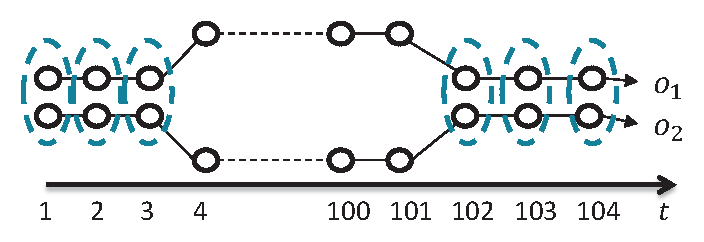
\includegraphics[width=0.5\textwidth]{platoon_weakpoint.eps}
\caption{Miss-pattern in platoon}
\label{fig:platoon_weakpoint}
\end{figure}

In platoon, a pattern for $n=2,k=4,l=2$ could be $\{o_1, o_2\}\{t_1,t_2,t_4,t_5,t_{100},t_{101}\}$. However, the snapshots $t_{100}$ and $t_{101}$ is too far away from previous snapshots. Such two snapshots are in less relation with previous snapshots and thus should be removed from the pattern. Based on this observation, we defined a \emph{generalized co-moving} pattern (as in Section~\ref{sec:definition}) to provide a more fine granular control of the pattern.
In \emph{generalized co-moving} pattern, a parameter $g$ is introduce the control the \emph{maximum gap} allowed between consecutive snapshots. By so doing our generalized co-moving pattern is more expressive and can represent all the existing co-moving patterns.

In step with the advances in localization technologies, the growth in the volume of trajectory data is rapid. Traditional single-machine methods face severe scalability problem in handling large trajectory data. For example, as reported in~\cite{li2015platoon}, a \emph{Swarm} pattern takes around 100 seconds to discover for 100k trajectories. With upto billions of trajectories in nowadays datasets, such approaches apparently become unfeasible. To tackle this challenge, we propose a 
paralleled solution for discovering \emph{generalized co-moving} patterns. We then deploy our idea on the modern MapReduce platform. As our experiments show, our solution achieves well load-balance and can process billions of trajectories in XXX seconds. Several optimizations are also designed to boost our solution to be orders of magnitudes faster than baseline algorithms.